%%%%%%%%%%%%%%%%%%%%%%%%%%%%%%%%%%%%%%%%%
% Beamer Presentation
% LaTeX Template
% Version 1.0 (10/11/12)
%
% This template has been downloaded from:
% http://www.LaTeXTemplates.com
%
% License:
% CC BY-NC-SA 3.0 (http://creativecommons.org/licenses/by-nc-sa/3.0/)
%
%%%%%%%%%%%%%%%%%%%%%%%%%%%%%%%%%%%%%%%%%

%----------------------------------------------------------------------------------------
%	PACKAGES AND THEMES
%----------------------------------------------------------------------------------------

\documentclass{beamer}

\mode<presentation> {

% The Beamer class comes with a number of default slide themes
% which change the colors and layouts of slides. Below this is a list
% of all the themes, uncomment each in turn to see what they look like.

%\usetheme{default}
\usetheme{AnnArbor}
%\usetheme{Antibes}
%\usetheme{Bergen}
%\usetheme{Berkeley}
%\usetheme{Berlin}
%\usetheme{Boadilla}
%\usetheme{CambridgeUS}
%\usetheme{Copenhagen}
%\usetheme{Darmstadt}
%\usetheme{Dresden}
%\usetheme{Frankfurt}
%\usetheme{Goettingen}
%\usetheme{Hannover}
%\usetheme{Ilmenau}
%\usetheme{JuanLesPins}
%\usetheme{Luebeck}
%\usetheme{Madrid}
%\usetheme{Malmoe}
%\usetheme{Marburg}
%\usetheme{Montpellier}
%\usetheme{PaloAlto}
%\usetheme{Pittsburgh}
%\usetheme{Rochester}
%\usetheme{Singapore}
%\usetheme{Szeged}
%\usetheme{Warsaw}

% As well as themes, the Beamer class has a number of color themes
% for any slide theme. Uncomment each of these in turn to see how it
% changes the colors of your current slide theme.

%\usecolortheme{albatross}
%\usecolortheme{beaver}
%\usecolortheme{beetle}
%\usecolortheme{crane}
%\usecolortheme{dolphin}
%\usecolortheme{dove}
%\usecolortheme{fly}
%\usecolortheme{lily}
%\usecolortheme{orchid}
%\usecolortheme{rose}
%\usecolortheme{seagull}
%\usecolortheme{seahorse}
%\usecolortheme{whale}
%\usecolortheme{wolverine}

%\setbeamertemplate{footline} % To remove the footer line in all slides uncomment this line
%\setbeamertemplate{footline}[page number] % To replace the footer line in all slides with a simple slide count uncomment this line

%\setbeamertemplate{navigation symbols}{} % To remove the navigation symbols from the bottom of all slides uncomment this line
}

\usepackage{graphicx} % Allows including images
\usepackage{booktabs} % Allows the use of \toprule, \midrule and \bottomrule in tables

%----------------------------------------------------------------------------------------
%	TITLE PAGE
%----------------------------------------------------------------------------------------

\title[Midterm Revision]{Exam Revision 3} % The short title appears at the bottom of every slide, the full title is only on the title page

\author{In Son Zeng} % Your name
\institute[University of Michigan] % Your institution as it will appear on the bottom of every slide, may be shorthand to save space
{
University of Michigan \\ % Your institution for the title page
\medskip
\textit{insonz@umich.edu} % Your email address
}
\date{\today} % Date, can be changed to a custom date

\begin{document}

\begin{frame}
\titlepage % Print the title page as the first slide
\end{frame}

\begin{frame}
\frametitle{Overview} % Table of contents slide, comment this block out to remove it
\tableofcontents % Throughout your presentation, if you choose to use \section{} and \subsection{} commands, these will automatically be printed on this slide as an overview of your presentation
\end{frame}

%----------------------------------------------------------------------------------------
%	PRESENTATION SLIDES
%----------------------------------------------------------------------------------------

%------------------------------------------------
\section{First Section} % Sections can be created in order to organize your presentation into discrete blocks, all sections and subsections are automatically printed in the table of contents as an overview of the talk
\subsection{Test Reminders}
\subsection{Videotaped Review and Solution}

%------------------------------------------------


\begin{frame}
\frametitle{Maximum Likelihood Estimator}

Step of deriving the Maximum Likelihood Estimator

\begin{enumerate}
\item Given $X_1, X_2,......X_n$ are i.i.d. random variables, we first find the joint PDF (likelihood function), which is $f(x_1, x_2,......, x_n;\lambda) = \prod_{i=1}^n f(x_i;\lambda)$. 

\item Take log for the likelihood function we obtain the log-likelihood function: $log\Big(f(x_1, x_2,......, x_n;\lambda)\Big)$

\item Then, we take the first derivative for the log-likelihood function with respect to the parameter of interest, and set to 0 (Maximizing): $\frac{\partial ln(f(x_1,x_2,......,x_n; \lambda}{\partial \lambda} = 0$. The solution of the equation is the candidate MLE $\hat \lambda$.

\item We take the second derivative $\frac{\partial^2 ln(f(x_1,x_2,......,x_n; \lambda}{\partial \lambda^2}$ and check whether it is less than 0. If yes, then the MLE is verified.

\end{enumerate}
\end{frame}

%------------------------------------------------

\begin{frame}
\frametitle{Invariance Principle of Maximum Likelihood Estimator}

This principal did not appear in the homework and Professor's exam review. But during the class he said we do need to know the Invariance Principle of MLE. Check the lecture notes and class note 13 for detail.

\begin{enumerate}
\item Given $X_1, X_2,......X_n$ are i.i.d. random variables. Suppose we have found that the MLE for $\lambda$ is $\hat \lambda$, then for any one-to-one transformation, say $\lambda \rightarrow g(\lambda)$, we can instantly recognize that the MLE of $g(\lambda)$ is $g(\hat \lambda)$.

\item Examples: For normal distribution $N(\mu,\sigma^2)$, we have found during the class that $\hat \sigma^2 = \frac{n-1}{n}S^2$, then since the domain of $\sigma^2 \in [0,\infty)$ and $\sigma \in [0,\infty)$, so $\hat \sigma = \sqrt{\frac{n-1}{n}S^2}$. (Here $g(x) = \sqrt{x}$)

\item Examples: Since the MLE for $\mu$ is $\bar X$, then by one-to-one transformation, the MLE for $\mu^5$ is $\bar X^5$, the MLE for $\mu^{\frac{1}{3}}$ is $\bar X^{\frac{1}{3}}$. With the same logic, what is the MLE for $\mu^3$ in the question? 

\end{enumerate}
\end{frame}

%------------------------------------------------
 



\begin{frame}
\frametitle{Test Reminders}

Let us be careful also about the following points during the exam 1:

\begin{enumerate}
\item You need to specify the
probability correctly. For example, "What is the probability that the reaction time for a randomly selected person is greater than 1.00 second?" Then you have to answer $P(X > 1.00)$. If the question becomes “greater than or equal to 1.00 second”
or “at least 1.00 second”, then you should answer $P(X \ge 1.00)$ to receive full credit.
\item To derive the standard deviation for the summation of independent random variables, say $X_1+X_2+......+X_n$,
please compute the variance first by formula $Var(X_1 + X_2 + ...... + X_n) = Var(X_1) + ...... + Var(X_n)$.
Then, you can take the square root to obtain the standard deviation. Do not directly add the standard
deviations.

\end{enumerate}
\end{frame}
%------------------------------------------------

\begin{frame}
\frametitle{Test Reminders}

Steps of constructing confidence interval for population mean:

\begin{enumerate}
\item The first step is the define the parameter correctly! The parameter should be the \textbf{population/true mean} of the subject mentioned in the question. 

\item The second step is to check \textbf{randomness} and Underlying population distribution (approximately) normal (\textbf{UPDN}) of the sample. First, we check whether the sample is random. If it is told, great! Just move on! If not, we can explain (most of the time) by your own reasoning why you think the collect sample is random or not.

\item Then, we check normality. If you are told UPDN, just proceed to next step. If not, then we check whether the sample size is large enough $n\ge 30$ to employ the CLT, which claims that the sampling distribution of the sample mean of the measurements is approximately normal. If the sample size is small $n<30$, then we rely on the robustness of the t procedures against violations of normality.

\end{enumerate}
\end{frame}
%------------------------------------------------

\begin{frame}
\frametitle{Test Reminders}

Steps of constructing confidence interval for population mean:

\begin{enumerate}
\item If $\sigma$ is given, skip this part. Otherwise, compute $s = \sqrt{\frac{1}{n-1}\sum_{i=1}^n (X_i - \bar X)^2}$, which is the square root of the sample variance.

\item \textbf{Computation} Find the t-score or z-score by referencing the table according to the specified significance level. For two-tails (keyword: \textbf{between},$\pm$ ) , we find $t_{\frac{\alpha}{2}}$ or $z_{\frac{\alpha}{2}}$; for one-tail (keyword: \textbf{no greater than, no less than}), we derive the confidence upper bound (CUB) or confidence lower bound (CLB) by finding $t_{\alpha}$ or $z_{\alpha}$

\item \textbf{Conclusion} We are approximately $100(1-\alpha) \%$ confident that the population mean of .....\underline{what \ question \ say}............ is (\underline{between /no greater than/no smaller than}) ...\underline{the \ confidence \ interval}....

\end{enumerate}
\end{frame}

%------------------------------------------------

\begin{frame}
\frametitle{Test Reminders}

Steps of performing hypothesis testing for population mean:

\begin{enumerate}
\item The first step is the define the parameter correctly! The parameter should be the \textbf{population/true mean} of the subject. 

\item The second step is the set up null hypothesis and alternative hypothesis. For two-tails, $H_0: \mu = \mu_0$ vs $H_1: \mu \ne \mu_0$ and for one-tail, we either 

\item The second step is to check \textbf{randomness} and Underlying population distribution (approximately) normal (\textbf{UPDN}) of the sample. 

\end{enumerate}
\end{frame}

%------------------------------------------------

\begin{frame}
\frametitle{Test Reminders}

Steps of performing hypothesis testing for population mean:

\begin{enumerate}
\item We specify the significance level $\alpha$, the values are usually 0.05 or 0.01.

\item We calculate the t-score with df $n-1$ by $t = \frac{\bar X - \mu_0}{s/\sqrt{n}}$

\item We check the t-table for the corresponding p-value given t-score you derived. If the question is asking two-tails, you need to multiply the p-value by 2. (No multiplication for one-tail)

\item Conclusion: With a p-value lower/greater than the significant level (such as 0.05, 0.01), we reject/fail to reject $H_0$. There is/is not sufficient evidence to suggest that the population mean of ...\underline{what \ question \ say}... is (\underline{different from/greater than/smaller than}) ...\underline{the \ number}....

\end{enumerate}
\end{frame}

%------------------------------------------------

\begin{frame}
\frametitle{Useful Links}

Let us watch some videos to revise the assumptions for various statistical concepts before the exam:

\begin{enumerate}


\item Coming soon!
\end{enumerate}
\end{frame}


%------------------------------------------------

\section{Second Section}
\subsection{Sample Questions}



%------------------------------------------------

\begin{frame}
\frametitle{Extra Questions}
\begin{block}{Question 1}

Let $X_1, X_2, ......, X_n$ be independent identically distributed random variables with common probability density function:

$$f(x_i;\theta) = (\theta+1) x_i^{\theta} \ 0\le \theta \le 1$$
and 0, otherwise. We typically know that the expectation and variance of $X_1,...X_n$ are identical.

a) First, compute $E(X_i)$ and $SD(X_i)$ for $i=1,2,...,n$.

b) Find the Maximum likelihood estimator of $\theta$

c) (Optional) Is the Maximum likelihood estimator of $\theta$ unbiased? Explain by showing the steps.

d) Find the Maximum likelihood estimator of $\theta^2$.

\end{block}


\end{frame}

%------------------------------------------------

\begin{frame}
\frametitle{Extra Questions}
\begin{block}{Question 1 Solution}

a) First, compute $E(X_i)$ and $SD(X_i)$ for $i=1,2,...,n$.

Sol: $E(X_i) = \int_0^1 x_i (\theta+1) x_i^{\theta} dx_i = \frac{\theta +1}{\theta+2}$, $E(X_i^2) = \int_0^1 x_i^2 (\theta+1) x_i^{\theta} dx_i = \frac{\theta +1}{\theta+3}$, then $SD(X_i) = \sqrt{E(X_i^2) - [E(X_i)]^2} = \sqrt{\frac{\theta +1}{\theta+3} - [\frac{\theta +1}{\theta+2}]^2}$

\vspace{3mm}

b) Find the Maximum likelihood estimator of $\theta$

Sol: $f(x_1,......,x_n;\theta) = (\theta+1)^n \cdot x_1^{\theta} \cdot ... \cdot x_n^{\theta}$, 0 otherwise. Take the log we get $log f(x_1,......,x_n;\theta) = n log(\theta+1) +  \theta(x_1 + ... + x_n)$. 

Take the first derivative we get $\frac{n}{\theta+1} + \sum_{i=1}^n log x_i = 0 \rightarrow \hat \theta = \frac{-n - \sum_{i=1}^n log x_i}{\sum_{i=1}^n log x_i}$.

To verify, we take the second derivative to get $-\frac{n}{(\theta+1)^2} <0$ so that the MLE for $\theta$ is $\hat \theta = -\frac{n}{\sum_{i=1}^n log x_i} - 1$

\end{block}
\end{frame}

%------------------------------------------------

\begin{frame}
\frametitle{Extra Questions}
\begin{block}{Question 1 Solution}

c) (Optional) Is the Maximum likelihood estimator of $\theta$ unbiased? Explain by showing the steps.

Come to my office hour because it is more challenging.

\vspace{3mm}

d) Find the Maximum likelihood estimator of $\theta^2$.

By the Invariance Principle of MLE, judging from the domain $0 \le \theta \le 1$, the transformation is one-to-one. Therefore, the MLE for $\theta^2$ is just the square of the MLE of $\theta$. Hence, $\hat \theta^2 = \frac{(-n - \sum_{i=1}^n log x_i)^2}{(\sum_{i=1}^n log x_i)^2}$

\end{block}

\end{frame}

%------------------------------------------------

\begin{frame}
\frametitle{Extra Questions}
\begin{block}{Question 2}
Recall that if $X_1,X_2,......,X_n$ are independent and normally distributed random variables with mean $\mu$ and variance $\sigma^2$, that is, $X_i \sim N(\mu,\sigma^2)$. 

\vspace{3mm}

a) Find the Maximum likelihood estimator for $\mu$.

b) Find the Maximum likelihood estimator for $\mu^3$.

c) Find the Maximum likelihood estimator for $\sigma^2$.

d) Let the Maximum likelihood estimator for $\sigma^2$ is $\hat \sigma^2$, find $E(\hat \sigma^2)$. 

e) Is the Maximum likelihood estimator for $\sigma^2$ unbiased? If not, then what should be the bias?

\end{block}


\end{frame}
%------------------------------------------------

\begin{frame}
\frametitle{Extra Questions}
\begin{block}{Question 2 Solution:}

a) Find the Maximum likelihood estimator for $\mu$.

c) Find the Maximum likelihood estimator for $\sigma^2$.

Sol: From the lecture notes, we have $f(x_1,......,x_n;\mu,\sigma^2) = \frac{1}{\sqrt{2\pi\sigma^2}} \cdot exp\Big(-\frac{1}{2\sigma^2}\sum_{i=1}^n(x_i - \mu)^2\Big)$. You can derive like the notes that $\hat \mu = \bar X$ and $\hat \sigma^2 = \frac{1}{n} \sum_{i=1}^n (X_i - \bar X)^2$

\vspace{3mm}
b) Find the Maximum likelihood estimator for $\mu^3$.

Sol: By the Invariance Principle, we take $g(x) = x^3$, so $\hat \mu^3 = (\bar X)^3$

\vspace{3mm}

d) Let the Maximum likelihood estimator for $\sigma^2$ is $\hat \sigma^2$, find $E(\hat \sigma^2)$. 

e) Is the Maximum likelihood estimator for $\sigma^2$ unbiased? If not, then what should be the bias? (Hint: $S^2 = \frac{1}{n-1}\sum_{i=1}^n (X_i - \bar X)^2$)

Sol: $E(\hat \sigma^2) = E(\frac{1}{n} \sum_{i=1}^n (X_i - \bar X)^2) = E(\frac{n-1}{n}S^2) = \frac{n-1}{n} \sigma^2$. Hence, the MLE of $\sigma^2$ is biased. The bias is $E(\hat \sigma^2) - \sigma^2 = -\frac{1}{n}\sigma^2$.

\end{block}


\end{frame}
%------------------------------------------------

\begin{frame}
\frametitle{Extra Questions}
\begin{block}{Question 3}
Suppose the nutrition label of apple cider says that apple cider contains an average concentration of 90 grams of sugar per liter, with standard deviation of  10 grams of sugar per liter. Now we want to check whether the claim is true. Therefore, we bought 50 liters of apple cider and found that 5050g sugar are contained in the 50 liters of apple cider in total. 

\vspace{5mm}
Based on this information, could we perform a hypothesis testing to check whether the claim in the nutrition label is true, at significance level $\alpha = 0.05$? If yes, please perform the hypothesis testing based on the steps taught in class. If not , please provide reason detailing why we could not perform such a hypothesis testing.

\end{block}
\end{frame}

%------------------------------------------------

\begin{frame}
\frametitle{Extra Questions}
\begin{block}{Question 3 Solution}

\begin{enumerate}
\item Let $\mu$ be the population mean concentration of sugar contained in a liter of apple cider.

\item The null hypothesis is $H_0: \mu = \mu_0 = 90$ grams versus $H_1 \ne 90$ grams.

\item Check randomness: the sample is not given random, but we believe that each liter of apple cider will not affect the other samples (independent).

\item Check UPDN: UPDN is not given. We check the sample size: $n = 50 \ge 30$, so we can use CLT and claim that the sample is approximately normal. We still use the t-test for the calculation given the degree of freedom $n-1 = 49$.

\end{enumerate}
\end{block}
\end{frame}

%------------------------------------------------

\begin{frame}
\frametitle{Extra Questions}
\begin{block}{Question 3 Solution}

\begin{enumerate}
\item We specify the significance level $\alpha = 0.05$. We also have known sample mean $\bar X = \frac{5050}{50} = 101$ grams/liter 

\item The t-statistics is: t = $\frac{\bar x - \mu_0}{\sigma/\sqrt{n}} = \frac{101 - 90}{10/\sqrt{50}} = 7.778$

\item By $1 - pt(7.778, 49)$ in R (Check the table during the test), and multiply the p-value by 2, we get the p-value $4.2 \times 10^{-10}$

\item Conclusion: Since the p-value is lower than 0.05, we reject the null hypothesis. There is sufficient evidence to suggest that the population mean concentration of sugar contained in a liter of apple cider is different from 90 grams/liter. 

\end{enumerate}
\end{block}
\end{frame}

%------------------------------------------------

\begin{frame}
\frametitle{Extra Questions}
\begin{block}{Question 4}
Suppose the nutrition label of apple cider says that apple cider contains an average concentration of 90 grams of sugar per liter, but the standard deviation is not given. Now we bought 10 liters of apple ciders instead, and found the concentrations of sugar for each liter of apple cider as follows: 95.3, 101.2, 92.3, 90.1, 96.4, 99.2, 110.3, 103.4, 91.2, 89.9. 

\vspace{5mm}
Based on this information, could we perform a hypothesis testing to check whether the claim in the nutrition label is true, at significance level $\alpha = 0.05$? If yes, please perform the hypothesis testing based on the steps taught in class. If not , please provide reason detailing why we could not perform such a hypothesis testing.

\end{block}
\end{frame}

%------------------------------------------------

\begin{frame}
\frametitle{Extra Questions}
\begin{block}{Question 4 Solution}

\begin{enumerate}
\item Again, let $\mu$ be the population mean concentration of sugar contained in a liter of apple cider.

\item The null hypothesis is $H_0: \mu = \mu_0 = 90$ grams versus $H_1 \ne 90$ grams.

\item Check randomness: the sample is not given random, but we believe that each liter of apple cider will not affect the other samples (independent).

\item Check UPDN: UPDN is not given. We check the sample size: $n = 10 \le 30$, so we cannot use CLT and claim that the sample is approximately normal. We need to rely on the robustness of t-test for the calculation given the degree of freedom $n-1 = 9$.

\end{enumerate}
\end{block}
\end{frame}

%------------------------------------------------

\begin{frame}
\frametitle{Extra Questions}
\begin{block}{Question 4 Solution}

\begin{enumerate}
\item We specify the significance level $\alpha = 0.05$. We also have known sample mean $\bar X = \frac{95.3 + ... + 89.9}{10} = 96.93$ grams/liter and sample standard deviation $s = \sqrt{\frac{1}{n-1}\sum_{i=1}^n (X_i - \bar X)^2} = 7.00$

\item The t-statistics is: $t = \frac{\bar x - \mu_0}{\sigma/\sqrt{n}} = \frac{96.93 - 90}{7.00/\sqrt{10}} = 3.13$

\item By $1 - pt(3.13, 9)$ in R (Check the table during the test), and multiply the p-value by 2, we get the p-value 0.0121.

\item Conclusion: Since the p-value is lower than 0.05, we reject the null hypothesis. There is sufficient evidence to suggest that the population mean concentration of sugar contained in a liter of apple cider is different from 90 grams/liter. 

\end{enumerate}
\end{block}
\end{frame}

%------------------------------------------------

\begin{frame}
\frametitle{Extra Questions}
\begin{block}{Question 5}
Many people are concerned that the average grade for STATS 250 in Winter 2018 semester was significantly lower than the average grade in previous semesters. Particularly, the grade distributions (assume that the first column is the Winter 2018 data, and the second column is the sample mean over 30 semesters) are as follows:

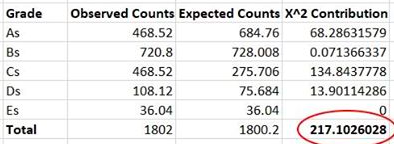
\includegraphics[width=0.9\textwidth]{250.png}

\end{block}
\end{frame}

%------------------------------------------------

\begin{frame}
\frametitle{Extra Questions}
\begin{block}{Question 5 (Continue)}

a) If the standard deviation of the number of students getting A's is 220, what is the 99 percent confidence interval of the true mean of the student getting the A's? (Since we have data from 30 semesters, the sample size should be 30 here)

b) What is the p-value of the 468.52 students getting A's in the Winter 2018 semester? What is the interpretation of such a p-value?

c) If the standard deviation of the number of students getting B's is 130, what is the 95 percent confidence interval of the true mean of the student getting the B's?

d) What is the p-value of the 720.8 students getting B's in the Winter 2018 semester? What is the interpretation of such a p-value?

e) Could we use the average grade of STATS 250 to make inference to the average grade of all classes in the University of Michigan? Why or why not?

\end{block}
\end{frame}

%------------------------------------------------

\begin{frame}
\frametitle{Extra Questions}
\begin{block}{Question 5 Solution:}

a) If the standard deviation of the number of students getting A's is 220, what is the 99 percent confidence interval of the true mean of the student getting the A's? (Since we have data from 30 semesters, the sample size should be 30 here)

b) What is the p-value of the 468.52 students getting A's in the Winter 2018 semester? What is the interpretation of such a p-value?

\begin{enumerate}

\item Let $\mu$ be the population mean number of students getting A's.

\item Check randomness: the sample is not given random, but we believe that each semester grade distribution will not affect the other samples (independent).

\item Check UPDN: UPDN is not given. We check the sample size: $n = 30 \ge 30$, so we can use CLT and claim that the sample is approximately normal. We still use the t-test for the calculation given the degree of freedom $n-1 = 29$.

\end{enumerate}
\end{block}
\end{frame}

%------------------------------------------------

\begin{frame}
\frametitle{Extra Questions}
\begin{block}{Question 5 Solution:}

\begin{enumerate}

\item From the technology $qt(0.995, 29) = 2.756$, we have the confidence interval $\bar x \pm t_{\frac{\alpha}{2},n-1} = 684.76 \pm 2.756 \cdot \frac{220}{\sqrt{30}} = 684.76 \pm 110.71 = (574.05, 795.47)$

\item Conclusion: Hence, we are approximately $99 \%$ confident that the population mean number of students getting A's is between 574.05 and 795.47 (approximately between 574 to 795 students).

\end{enumerate}
\end{block}
\end{frame}
%------------------------------------------------

\begin{frame}
\frametitle{Extra Questions}
\begin{block}{Question 5 Solution:}

\begin{enumerate}

\item With the same setting, $t = \frac{\bar x - \mu}{\sigma/\sqrt{n}} = \frac{468.52 - 684.76}{220/\sqrt{30}} = -5.384$.

\item From technology, the corresponding p-value is $4.37 \times 10^{-6}$ (lower-tail), which means that the probability of observing a semester with 468.52 or even less students getting A's in STATS 250 is $4.37 \times 10^{-6}$.

\item Alternatively, we can use two-tail, which gives p-value $8.74 \times 10^{-6}$, which means that the probability of observing a semester as extreme as, or more extreme than, 468.52 students getting A's in STATS 250 is $8.74 \times 10^{-6}$.

\end{enumerate}
\end{block}
\end{frame}

%------------------------------------------------

\begin{frame}
\frametitle{Extra Questions}
\begin{block}{Question 5 Solution:}

c) If the standard deviation of the number of students getting B's is 130, what is the 95 percent confidence interval of the true mean of the student getting the B's?

d) What is the p-value of the 720.8 students getting B's in the Winter 2018 semester? What is the interpretation of such a p-value?

\begin{enumerate}

\item Let $\mu$ be the population mean number of students getting B's.

\item Check randomness: the sample is not given random, but we believe that each semester grade distribution will not affect the other samples (independent).

\item Check UPDN: UPDN is not given. We check the sample size: $n = 30 \ge 30$, so we can use CLT and claim that the sample is approximately normal. We still use the t-test for the calculation given the degree of freedom $n-1 = 29$.

\end{enumerate}
\end{block}
\end{frame}

%------------------------------------------------

\begin{frame}
\frametitle{Extra Questions}
\begin{block}{Question 5 Solution:}

\begin{enumerate}

\item From the technology $qt(0.975, 29) = 2.045$, we have the confidence interval $\bar x \pm t_{\frac{\alpha}{2},n-1} = 728.008 \pm 2.045 \cdot \frac{130}{\sqrt{30}} = 728.008 \pm 48.537 = (679.47, 776.55)$

\item Conclusion: Hence, we are approximately $95 \%$ confident that the population mean number of students getting B's is between 679.47 and 776.55 (approximately between 679 to 777 students).

\end{enumerate}
\end{block}
\end{frame}
%------------------------------------------------

\begin{frame}
\frametitle{Extra Questions}
\begin{block}{Question 5 Solution:}

\begin{enumerate}

\item With the same setting, $t = \frac{\bar x - \mu}{\sigma/\sqrt{n}} = \frac{720.8 - 728.008}{130/\sqrt{30}} = -0.304$.

\item From technology, the corresponding p-value is $0.382$ (lower-tail), which means that the probability of observing a semester with 728.008 or even less students getting B's in STATS 250 is $0.382$.

\item Alternatively, we can use two-tail, which gives p-value $0.764$, which means that the probability of observing a semester as extreme as, or more extreme than, 728.008 students getting B's in STATS 250 is $0.764$.

\end{enumerate}
\end{block}
\end{frame}

%------------------------------------------------

\begin{frame}
\frametitle{Extra Questions}
\begin{block}{Question 5 Solution:}

e) Could we use the average grade of STATS 250 to make inference to the average grade of all classes in the University of Michigan? Why or why not?
\begin{enumerate}

\item The students studying STATS 250 only represents a subset of population, which is all students in University of Michigan. Therefore, we cannot use the average grade of STATS 250 to make inference to the population mean grade of all class in the University of Michigan.

\end{enumerate}
\end{block}
\end{frame}
%------------------------------------------------

\begin{frame}
\frametitle{Extra Questions}
\begin{block}{Question 6 }

More questions are coming soon for CLT and distributions.

Good luck I tried my really best...

\end{block}
\end{frame}

%------------------------------------------------

\begin{frame}
\frametitle{Go Wolverines!}

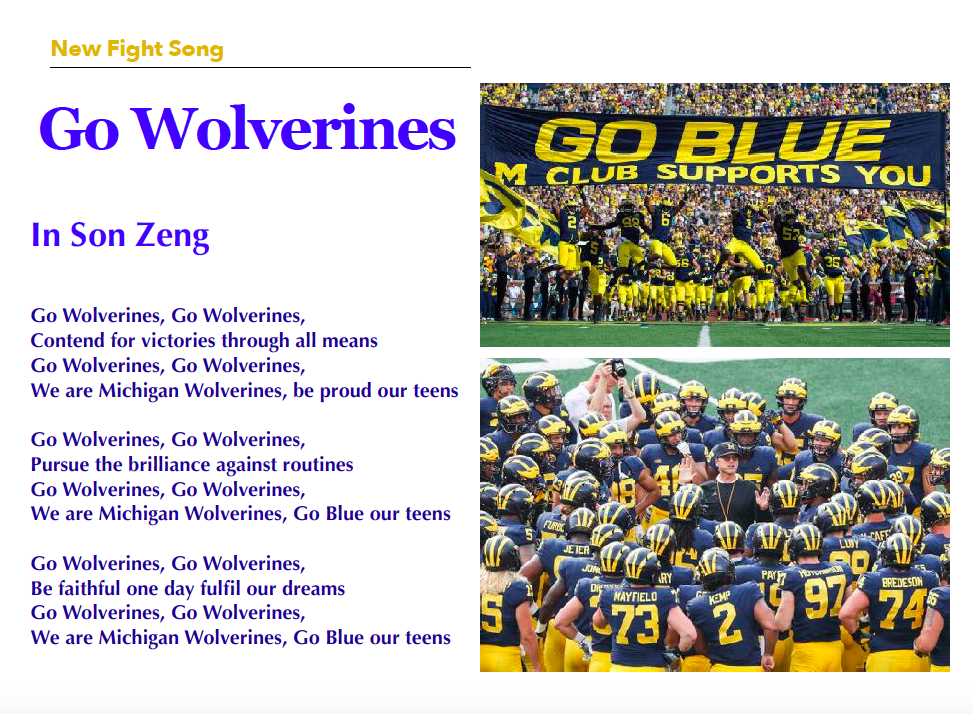
\includegraphics[width=0.85\textwidth]{Go Wolverines.png}

\end{frame}

%------------------------------------------------
\begin{frame}
\Huge{\centerline{The End}}
\end{frame}

%----------------------------------------------------------------------------------------

\end{document}